\chapter{}\label{ex:aufg2}

\section{}\label{sec:aufg2a}
Gegeben ist Strangwiederstand $R_S = 2.32 \Omega$ und eine Stranginduktivität $L_S= 11.4$mH.
Mit der Formel aus dem Skript
\begin{equation}
	U_S = R_S * I_S + L_S * \frac{dI_S(t)}{dt} + U_{iS}
\end{equation}
und $U_{iS} = 0$ bekommt man als Lösung der Differantialgleichung
\begin{equation}
	I_S = \frac{U_S}{R_S}~( 1 - e^{-\frac{t}{\tau}})
\end{equation}
mit $\tau = \frac{L_S}{R_S} = 4.91$ms und eingesetzten Werten ergibt sich folgender Stromverlauf(siehe Abb. \ref{fig:2a_stromverlauf_I1}).
\begin{figure}[htb]
	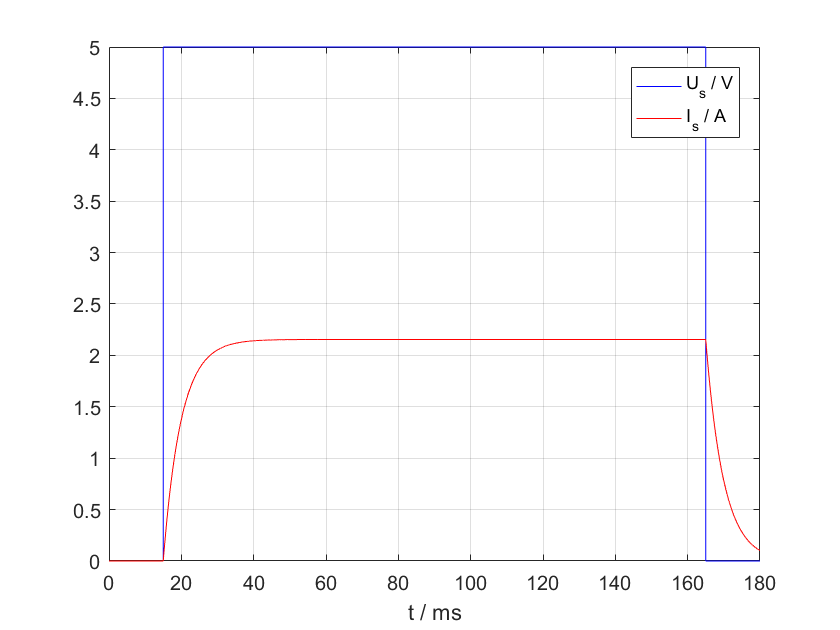
\includegraphics[width=\textwidth]{./Bilder/2a_Stromverlauf_1}
	\caption{Stromverlauf der $I_1$}
	\label{fig:2a_stromverlauf_I1}
\end{figure}

\begin{figure}[htb]
	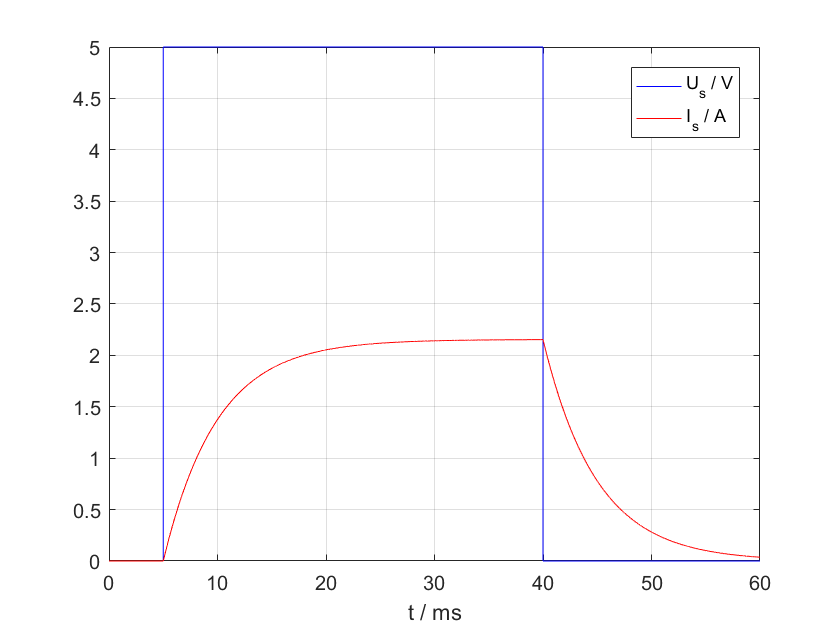
\includegraphics[width=\textwidth]{./Bilder/2a_Stromverlauf_2}
	\caption{Stromverlauf der $I_2$}
	\label{fig:2a_stromverlauf_I2}
\end{figure}

\begin{figure}[htb]
	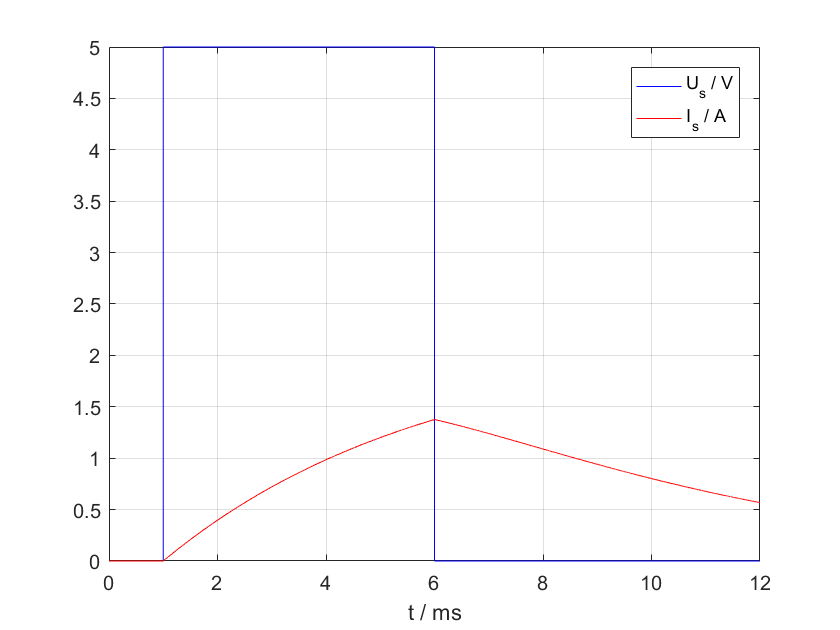
\includegraphics[width=\textwidth]{./Bilder/2a_Stromverlauf_3}
	\caption{Stromverlauf der $I_3$}
	\label{fig:2a_stromverlauf_I3}
\end{figure}

\section{}\label{sec:aufg2b}


\clearpage